Os documentos a seguir estão disponíveis no repositório do projeto~\cite{ref:github_soe}, servem como documentação local do repositório e estão sendo apresentados como apêndices a esse trabalho:
\section*{Apêndice}

\begin{itemize}

    \item \textbf{Apêndice A --- Descrição das Peças} --- descrição de cada peça mecânica fabricada por impressão 3D para a esteira, incluindo função e quantidade.

    \item \textbf{Apêndice B --- Fechamento do Escopo} --- documento que concentra de forma sucinta o contexto de aplicação, os objetivos, as limitações e as referências bibliográficas do projeto.

    \item \textbf{Apêndice C --- Esquemático da placa com STM32G070}

\end{itemize}

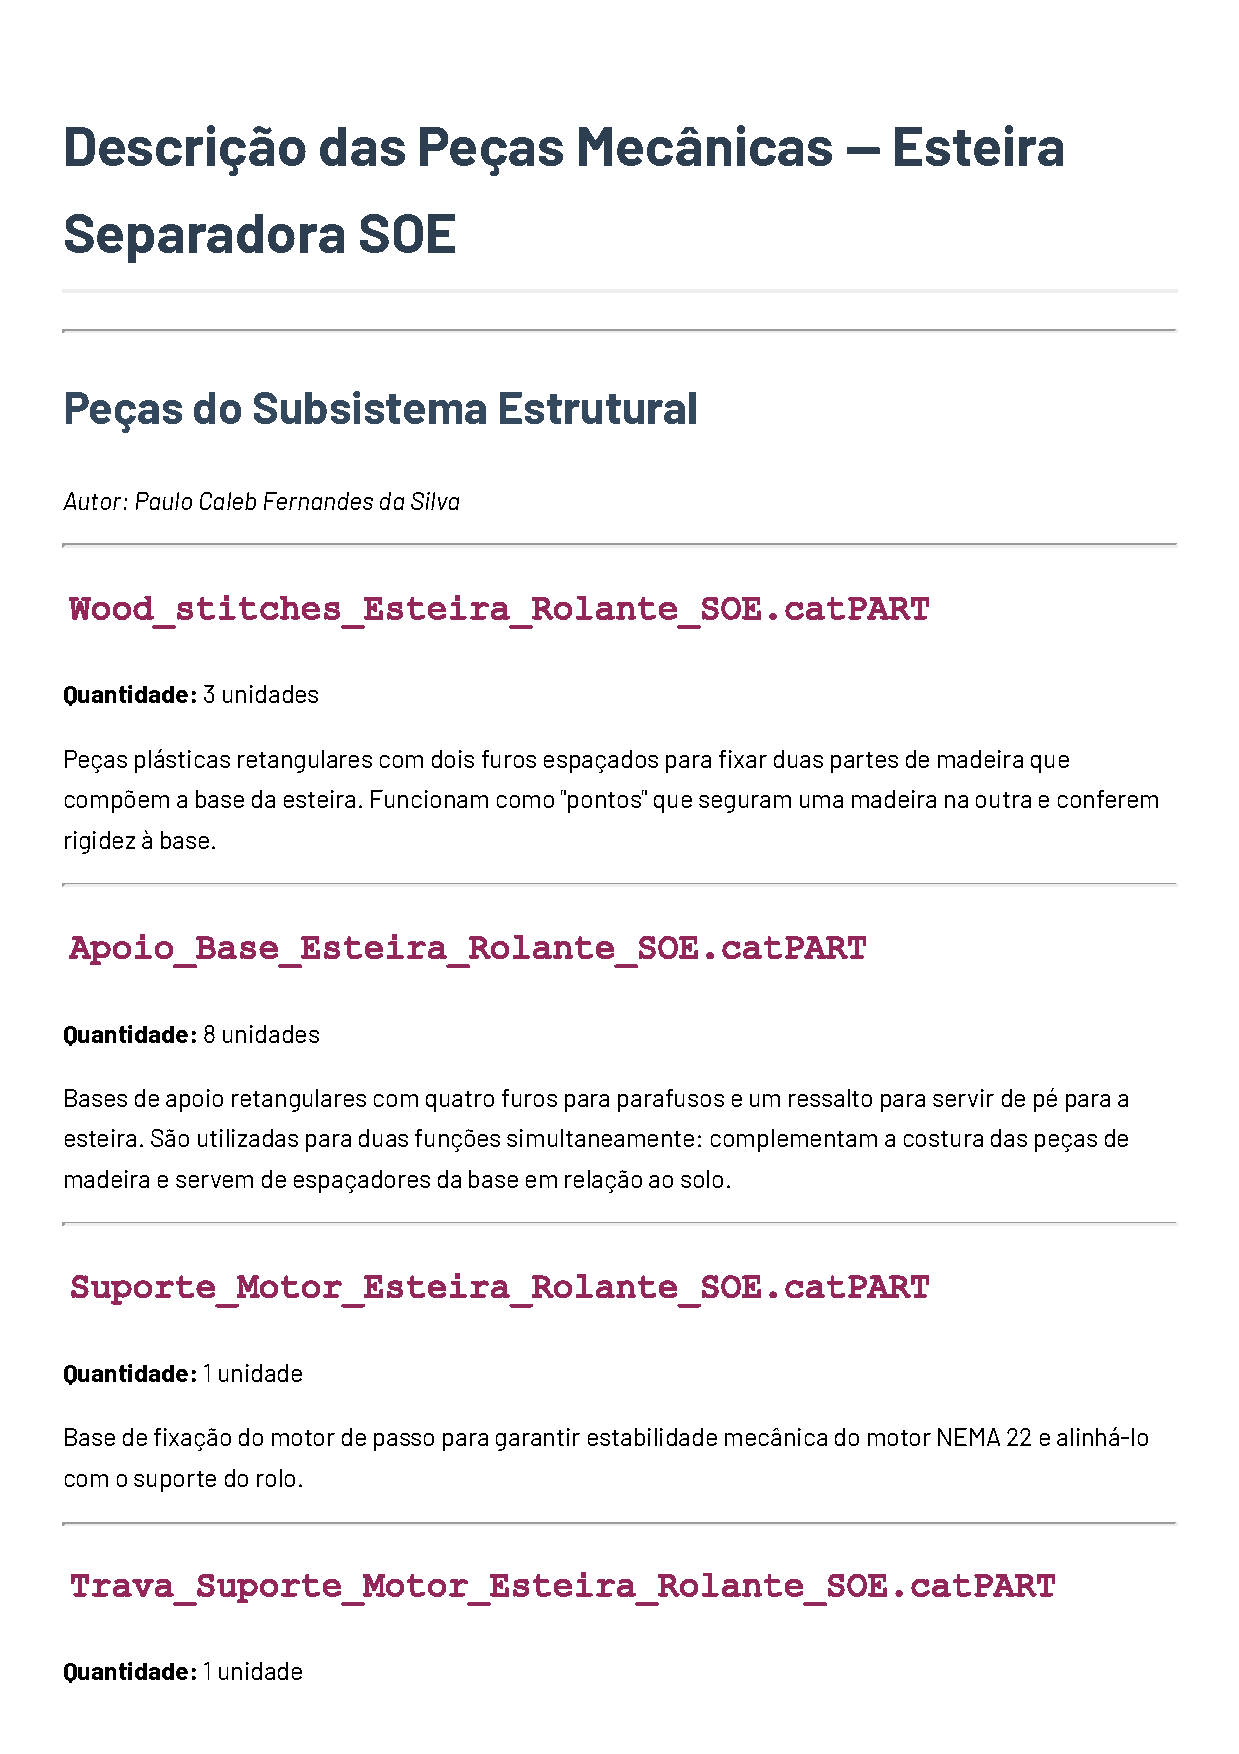
\includepdf[pages=-, pagecommand={\thispagestyle{plain}}]
           {pdfs/Descricao_das_pecas.pdf}

\newpage

\section*{Fechamento do Escopo -- Projeto Final SOE}

% ------------------------------------------------------------------
\subsection*{1. Contexto de Aplicação}

Sistemas de logística interna em centros de distribuição utilizam linhas
automatizadas de transporte e separação de itens para preparação de pedidos.
Esses sistemas são compostos por módulos de esteiras interconectados, capazes
de identificar e direcionar produtos conforme seu destino.

% ------------------------------------------------------------------
\subsection*{2. Definição do Problema}

Dado um fluxo contínuo de itens previamente identificados, é necessário
desenvolver um módulo de esteira automatizado capaz de:

\begin{itemize}
    \item Permitir a identificação de cada item;
    \item Determinar o destino de cada item;
    \item Direcioná-lo corretamente dentro de uma linha de separação modular.
\end{itemize}

% ------------------------------------------------------------------
\subsection*{3. Objetivo do Projeto}

Desenvolver um sistema embarcado para controle de um módulo de esteira
automatizada com capacidade de identificação e desvio de itens de acordo com o
destino previamente associado ao objeto, com ênfase na integração entre
controle embarcado e processamento em sistema Linux embarcado.

\subsubsection*{Objetivos Específicos}

\begin{itemize}
    \item Implementar controle de movimentação da esteira;
    \item Desenvolver mecanismo de desvio de itens;
    \item Integrar comunicação com sistema externo;
    \item Validar o funcionamento do sistema experimentalmente.
\end{itemize}

% ------------------------------------------------------------------
\subsection*{4. Escopo do Sistema}

O sistema consiste em um módulo de esteira com:

\begin{itemize}
    \item 1 entrada de itens;
    \item 2 saídas (desvio local ou encaminhamento para próximo módulo).
\end{itemize}

Capaz de operar com objetos que atendam às seguintes restrições:

\begin{itemize}
    \item Massa máxima: 250\,g;
    \item Volume máximo: 125\,cm³;
    \item Altura: entre 2\,cm e 5\,cm.
\end{itemize}

% ------------------------------------------------------------------
\subsection*{5. Funcionalidades do Sistema}

O sistema embarcado deverá:

\begin{enumerate}
    \item Detectar a presença de objetos na esteira;
    \item Controlar o deslocamento do item até a zona de leitura;
    \item Solicitar ao servidor, via interface de comunicação, a identificação
          do item;
    \item Receber do servidor a decisão de destino;
    \item Executar o desvio do item para uma das saídas.
\end{enumerate}

% ------------------------------------------------------------------
\subsection*{6. Interface com o Servidor (ex.: Raspberry Pi)}

O módulo deverá possuir interface de comunicação com um servidor que será
responsável por:

\begin{itemize}
    \item Captura de imagem do item na zona de leitura;
    \item Processamento e decodificação do código QR;
    \item Determinação do destino do item;
    \item Envio de comandos ao módulo da esteira;
    \item Monitoramento do estado do sistema;
    \item Registro de eventos de operação.
\end{itemize}

% ------------------------------------------------------------------
\subsection*{7. Limitações do Projeto}

Este projeto não contempla:

\begin{itemize}
    \item Integração com sistemas reais de estoque;
    \item Implementação de múltiplos módulos interconectados;
    \item Processamento de múltiplos itens simultaneamente;
    \item Sistemas avançados de visão computacional.
\end{itemize}

% ------------------------------------------------------------------
\subsection*{8. Resultados Esperados}

\begin{itemize}
    \item Protótipo funcional de um módulo de esteira automatizado validado
          experimentalmente;
    \item Sistema embarcado operando integrado a um ambiente Linux embarcado;
    \item Capacidade de identificação e separação de itens conforme o destino
          definido;
    \item Documentação técnica completa do sistema.
\end{itemize}

% ------------------------------------------------------------------
\subsection*{9. Aplicação}

O sistema proposto se aplica a processos de automação logística em centros de
distribuição, podendo ser utilizado como base para sistemas modulares escaláveis
de separação de pedidos. A arquitetura proposta segue o modelo de processamento
distribuído, separando tarefas de tempo real e processamento de alto nível.

% ------------------------------------------------------------------

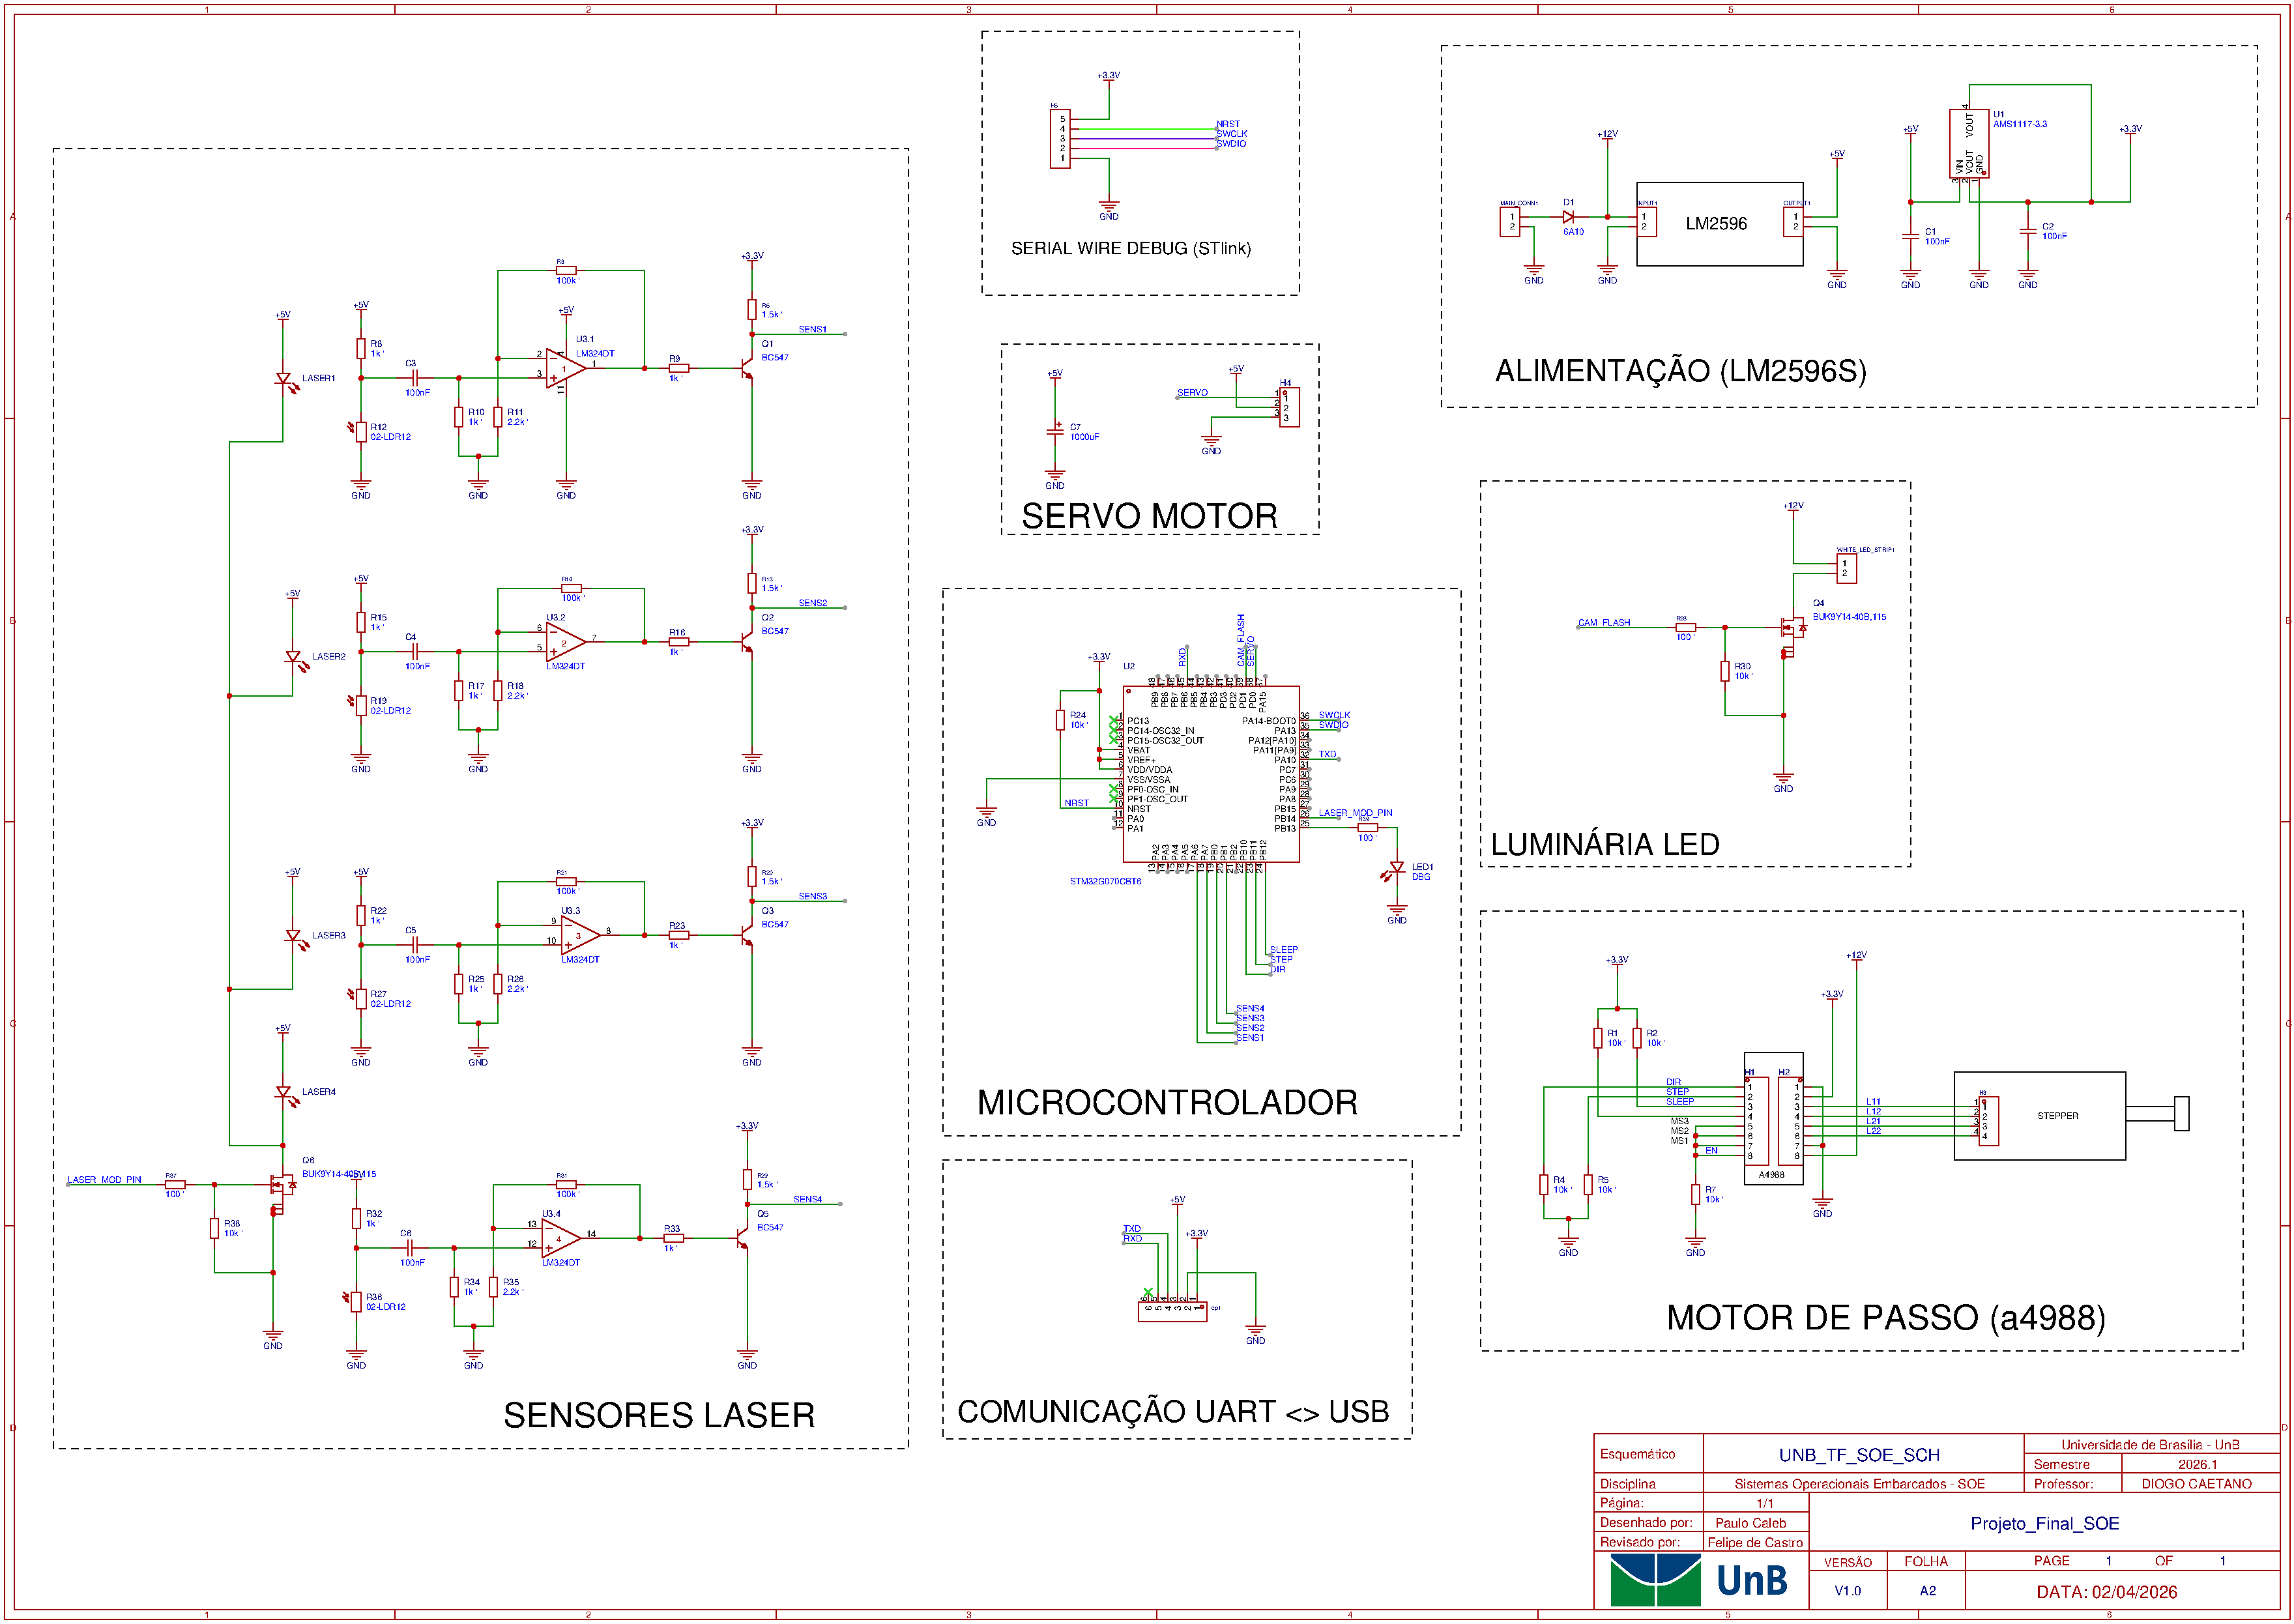
\includepdf[pages=-, pagecommand={\thispagestyle{plain}}]
           {pdfs/SCH_UNB_TF_SOE_SCH_2026-06-12.pdf}